\chapter{Podstawy teoretyczne}
\label{ch:podstawy-teoretyczne}

W niniejszym rozdziale przedstawiono kluczowe zagadnienia teoretyczne, które stanowią fundament techniczny realizowanego projektu. Przedstawienie podstaw działania zastosowanych elementów pozwoli lepiej zrozumieć wyzwania projektowe oraz przyjęte metody rozwiązywania problemów związanych ze sterowaniem i nawigacją mobilnej platformy robotycznej. 

Omówione zostaną najważniejsze zasady funkcjonowania enkoderów kwadraturowych, które umożliwiają dokładne monitorowanie ruchu - podstawowej odometrii. Zaprezentowane zostaną także zasady działania regulatora PID, powszechnie stosowanego w układach sterowania, który pozwala na kontrolowanie prędkości obrotowej silników. W dalszej części omówiono wybrane algorytmy z zakresu wizji komputerowej, takie jak detekcja krawędzi i rozpoznawanie kolorów, które stanowią istotne elementy systemu wizyjnego robota.

\section{Enkodery}

Enkodery są urządzeniami pomiarowymi, które umożliwiają śledzenie ruchu obrotowego lub liniowego i są nieodzownym elementem systemów sterowania oraz automatyzacji. W zastosowaniach robotycznych, takich jak opisywana platforma mobilna, enkodery umożliwiają śledzenie prędkości i pozycji, co jest kluczowe dla poprawnej implementacji odometrii – procesu śledzenia pozycji robota w przestrzeni. Enkodery dzielą się na enkodery optyczne, magnetyczne i mechaniczne, w zależności od zastosowanej technologii detekcji. W omawianym projekcie szczególne zastosowanie znajdują enkodery kwadraturowe, montowane przy silnikach odpowiedzialnych za napęd różnicowy robota.

\subsection{Enkodery kwadraturowe}

Enkodery kwadraturowe to specjalny rodzaj enkoderów, które umożliwiają nie tylko pomiar prędkości i położenia, ale także kierunku obrotu. Składają się z dwóch sygnałów wyjściowych – A i B – przesuniętych względem siebie o fazę 90°. Dzięki temu fazowemu przesunięciu system sterujący jest w stanie określić kierunek obrotu, analizując, który z sygnałów A lub B wyprzedza drugi. Każdy impuls generowany przez sygnały A i B odpowiada określonemu przemieszczeniu kątowemu, co pozwala na wyznaczenie pozycji kątowej osi obrotu z wysoką precyzją. Przy odpowiednim przetwarzaniu sygnałów z enkoderów kwadraturowych możliwe jest uzyskanie wysokiej rozdzielczości pomiaru pozycji, co ma istotne znaczenie przy realizacji odometrii robota.

\subsubsection{Efekt Hall'a}



\begin{figure}[h]
    \centering
    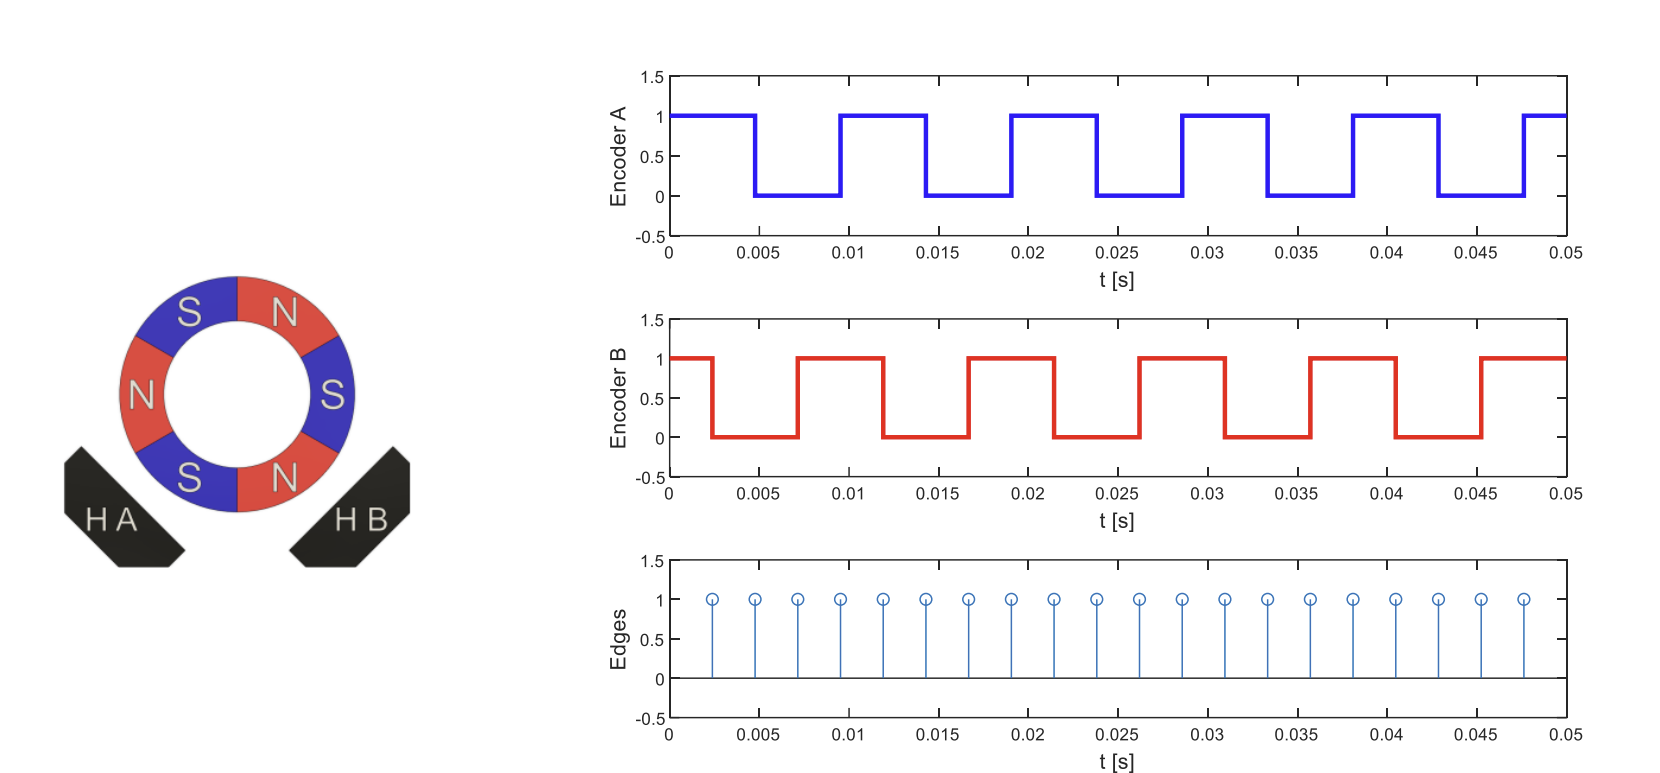
\includegraphics[width=1.0\textwidth]{./graf/enkoders.png}
    \caption{Rysunek przedstawiający ideowo budowę enkodera kwadraturowego oraz sygnałów przez niego generowanych - źródło \cite{bib:encoders-pid}}
    \label{rys2:encoders-graf}
\end{figure}

\subsection{Enkodery kwadraturowe w odometrii}

W kontekście omawianego projektu enkodery kwadraturowe zamontowane na osiach napędowych pozwalają na ciągłe śledzenie ruchu robota i na podstawie liczby impulsów na wyjściach A i B umożliwiają obliczanie dystansu, jaki przebył robot, oraz jego prędkości. Względne przesunięcie fazowe sygnałów z enkodera informuje o kierunku ruchu, a liczba impulsów na jednostkę obrotu pozwala na bardzo dokładne określenie przebytej odległości. Wykorzystanie enkoderów kwadraturowych znacznie poprawia dokładność odometrii, co ma kluczowe znaczenie dla lokalizacji robota w przestrzeni oraz realizacji zaplanowanej trajektorii.

\section{Regulator PID}


\section{Podstawy wykrywania krawędzi w wizji komputerowej}


\section{Podstawy rozpoznawania kolorów w wizji komputerowej}

